\documentclass{article}
\usepackage[utf8]{inputenc}
\usepackage{amsmath}
\usepackage{amssymb}
\usepackage{svg}
\usepackage{showlabels}
\usepackage{comment}
\usepackage{cite}
\usepackage{notoccite}
\usepackage{subfig}

\usepackage{dsfont}

\title{Bachelor}
\author{Lars Müller}
\date{February 2022}

\begin{document}

\maketitle

\section{Abstract}
In this work I combine recent advances in unsupervised reinforcement learning with the objectives of Phasic Policy Gradient (PPG).
Active Pre-Training (APT) is used to train an agent with intrinsic reward based on the particle based entropy to latent representations
of the k-nearest neighbors. These latent representations are learned via contrastive learning.
After pre training in such manner, one defines a downstream task via exposing the model free algorithm to a task specific reward function.
Then the pre-trained agent can be compared to vanilla agent when exposed to a downstream reward.
This is done in a sparse and dense reward setting.


\section{Introduction}

Machine Learning and its sub-fields deep learning and reinforcement learning have seen
a rise in popularity in the recent years.
Since AlexNET~\cite{NIPS2012_c399862d} neural networks became essential to
most machine learning tasks, as they require less expert knowledge and are
more flexible~\cite{DBLP:journals/corr/abs-1910-13796}. The upcoming of deep learning
and neural networks as their backbone have transformed the field and allows to approach
a wider variety of tasks.\\
Deep learning has found application in many widely used products such as recommendation engines or drug discovery. Reinforcement learning
is not as commonly encountered, but is still used in robotic manipulation tasks or other
control-over-time related tasks. This is due to a variety of factors such as the complexity of deep reinforcement learning systems in comparison to systems that operate on a static data set.
Robotic tasks such as Dexterous In-Hand Manipulation~\cite{DBLP:journals/corr/abs-1808-00177}
have been solved. The industry uses a variety of research~\cite{DBLP:journals/corr/abs-1710-04615}~\cite{Li2020Sub-policy}~\cite{DBLP:journals/corr/abs-1803-05268}
to engineer robots used to automatically solve pick and place tasks in real world environments.
These robots are put to work in warehouses or other difficult environments to work with minimal
human intervention.\\
To test which methods work best a lot of benchmarks are performed on the Atari benchmark~\cite{DBLP:journals/corr/abs-1207-4708},
which will be used to evaluate performance in this thesis too.
This introduction explains the basics of neural networks and the training
procedure.

\subsection{Fully connected layer}
A single layer perceptron or fully connected layer is an affine function of the form 
\begin{equation}
    \eta: 	\mathbb{R}^n \xrightarrow{} \mathbb{R}^m
\end{equation}
\begin{equation*}
    \eta(x; W, b) = x W^T + b
\end{equation*}
where $x\in \mathbb{R}^{1 \times n} $, $W\in \mathbb{R}^{m \times n}$ and $ b \in \mathbb{R}^{1 \times m}$.
This is usually~\cite{kulathunga2020effects} followed by a nonlinear function $\phi$. This so-called activation function allows us
to model nonlinearities in the data and approximate more complex functions.\\

\noindent In a multilayer perceptron $N$ single layer perceptrons are stacked and iteratively transform an input $x_0$. 
Each layer $h_i, i \in \{1, ..., N\}$ is parametrized by the weight matrix $W_i$ and bias vector $b_i$ and computes
the input $x_i$ for the next layer. Layer $h_i$ is defined as:

\begin{equation}
    h_i: \mathbb{R}^n \xrightarrow{} \mathbb{R}^m
\end{equation}
\begin{equation*}\
    h_i(x_{i-1}; W_i, b_i) = \phi(\eta(x_{i-1}; W_i, b_i))
\end{equation*}
 
\noindent Multilayer perceptrons (MLP) are a class of feed-forward neural networks.
\begin{figure}[htbp]
  \centering
  \includesvg[width = 150pt]{nn.svg}
  \caption{MLP Visualization for N = 3}
\end{figure}

\subsection{Convolution layer}
\noindent One can also replace the single layer perceptron with a convolution layer because they have some
favorable properties such as less required compute. 

\noindent Convolution layers are well suited for images where the input is now a tensor
of shape $x \in \mathbb{R}^{c \times n \times m}$, with $c = 3$ for colored
picture. Each dimension represents a color channel of red, blue and yellow and
can contain integer values from 0 to 255. For illustration purposes I will assume
a gray-scale image with only one channel, or $c = 1$.

\noindent Each convolution layer has filters or kernel $f_i \in \mathbb{R}^{q \times r}$ and each $f_i$ has a bias $b_i \in \mathbb{R}$.
These filters are moved over the input image by first positioning the top left corner of the filter matrix at the top left of the input matrix and act as the weights $\theta$ of the layer.
The filter matrix and the corresponding image section are then multiplied element-wise and
the filter is moved. The new position of the filter is determined by the stride parameter, which specifies how many pixels we move the filter to the right and how many pixels we move it down.
For each feature map there will be kernels applied to the corresponding image channel which are then concatenated by adding them. This means for $c > 1$ $f_i$s dimension will increase equally.\\
\noindent For notation purpose I will include the matrix indices in the exponent where $f_i^{j,k}$ refers
to the $j$'th row and the $k$'th column of $f_i$. For every filter $f_i$ a result Matrix $M_i \in \mathbb{R}^{o \times p}$ is created, whose rows and columns
will be indexed by $J$ and $K$ respectively. 

\begin{equation}
    conv: \mathbb{R}^{n \times m} \xrightarrow{} \mathbb{R}^{o \times p}
\end{equation}
\begin{equation*}
    M_i^{J, K} = conv(x, J, K; f_i, b_i) = b_i + \sum_{j=0}^{q-1} \sum_{k=0}^{r-1} f_i^{j,k} x^{J+j, K+k}
\end{equation*}

\noindent This can be repeated for each layer, for multiple $f_i$ operating on multiple $M_j$, where $M$ is commonly
referred to as feature map.
Due to their spatial invariance convolution layers see lots of popularity, especially on image data~\cite{DBLP:journals/corr/abs-2002-02959}. 
Perceptron and convolution layers can be combined in neural network architectures by reshaping the data when transitioning between them. Convolution layers usually use a Rectified Linear Unit (ReLU)~\cite{DBLP:journals/corr/abs-1803-08375} as their nonlinearity because of its favorable properties such as non-saturation of its gradient and low compute cost.\newline

\begin{figure}[htbp]
  \centering
  \includesvg[width = 250pt]{convn.svg}
  \caption{Visualization of an example neural network}
\end{figure}

\subsection{Activation functions}

\noindent The first layer is referred to as the input layer and the last one as the output layer. Layers between
these are called hidden layers.

\begin{equation}
    ReLU: \mathbb{R}^{n \times m} \xrightarrow{} \mathbb{R}^{n \times m}
\end{equation}
\begin{equation*}
    ReLU(x)=
        \begin{cases}
            0 &x\leq 0 \\
            x&\text{otherwise}
        \end{cases}
\end{equation*}

\noindent A common choice for the nonlinearity of the output layer is the $softmax$ function  to convert the 
logits that network outputs to a probability distribution. 

\begin{equation}
    softmax: \mathbb{R}^K \xrightarrow{} \mathbb{R}^K
\end{equation}
\begin{equation*}
    softmax(x) = \frac{e^{y_j}}{\sum_{k=1}^K e^{y_k}}
\end{equation*}

where $K$ is the the dimension after the output layer.

\noindent A probability distribution as an output of the neural network is commonly used in multiclass classification.
A distribution can be used to determine how confident as neural network classifies a given input.
Low entropy of the distribution of $softmax(x)$ indicates a high confidence, while a high entropy
indicates a uniform distribution over the classes and therefore a low confidence.\\

\subsection{Training and loss functions}
\noindent Neural networks are updated via Stochastic Gradient Descent on a loss function that defines the objective.
The gradient w.r.t. the parameters $\theta$ of the neural network is used to update the parameters of the network with an optimization algorithm e.g. ADAM. This is done on subsets of the data, called mini batches.\\

\noindent Let $\phi_\theta: \mathbb{R}^{c \times n \times m} \xrightarrow{} \mathbb{R}^{k \times l}$ be a neural network consisting of a combination of convolution and fully connected layers which is parametrized by $\theta$.

\noindent To calculate the mean squared error loss $MSE$, 
we need our predicted value $\hat y \in \mathbb{R}^{n}$ and the true
label or the value you want to fit the network on $y \in \mathbb{R}^{n}$.
The output of our neural network $\phi_\theta(x)$ will be called $\hat{y}$. 
Mean squared error is mostly used in regression.

\begin{equation}
    MSE: \mathbb{R}^{n \times n} \xrightarrow{} \mathbb{R}
\end{equation}
\begin{equation*}
    MSE(y, \hat{y}) = \frac{1}{n} \sum_{i=0}^{n} (y_i-\hat{y}_i)^2
\end{equation*}

\noindent Another important loss is the cross-entropy loss $ce$. It is mainly used for multiclass classification and expects
probabilities over $k$ classes, so softmax is usually applied as the non-linearity of the output layer.
$y \in \{0, 1\}^{k}$ is a vector that contains the true class labels. $p \in [0, 1]^{k}$ contains
the per class probabilities that $\phi_\theta(x)$ predicts.
\begin{equation}
    ce: \mathbb{R}^{k} \xrightarrow{} \mathbb{R}
\end{equation}
\begin{equation*}
    ce(y, p) = \sum_{c=1}^My_{i}\log(p_{i})
\end{equation*}

\noindent If vanilla stochastic gradient descent is used as the optimization algorithm, the weights $\theta$
are updated via 
\begin{equation}
    \theta \xleftarrow{} \theta + \nabla_\theta {\mathcal L}(y, \phi_\theta(x))
\end{equation}
on the chosen loss ${\mathcal L}$.

\noindent In supervised learning $y$ is either obtainable by labeling data by hand or given
by some other source. If this is not an option different methods from
self-supervised and unsupervised learning can help create a target $y$.\newline
Unsupervised learning attempts to find patterns and group inputs that can then be 
interpreted as belonging to a category or label.
Self supervised learning is a more direct approach to form targets.

\section{Self supervised learning}
For problems where data labeling is not feasible self-supervised learning or SSL
provides a way to obtain target and fit a neural network on those. SSL also enables us
to pretrain neural networks and then switch to a downstream task by exposing the
supervised labels to it and fine tune the neural network on them. SSL autonomously creates
labels by using information from domain knowledge or correlations.\newline

\subsection{SimCLR}

SimCLR~\cite{DBLP:journals/corr/abs-2002-05709} is a contrastive self-supervised framework which stands for simple framework for contrastive learning of visual representations.
This framework defines the following components, which aim to learn  meaningful vector representations of images.\\
At first a task-specific data augmentation module is defined. Data augmentations can have a significant impact on performance and it is important that they do not change the semantic meaning of the images. 
Multiple augmentations such as gaussian blur, cropping and resizing are applied sequentially to the input image.\\
Then a neural network architecture is selected as an encoder.
The authors use the ResNet~\cite{he2015deep} architecture for this purpose, more precisely the output of the average pooling layer denoted as $h_i = f(\tilde{x_i})$ where $\tilde{x_i}$ is an augmented image view. $h_i$ is the learned representation and consists of
high level features.\\
On top of their encoder they add a two layer MLP with a ReLU activation in between which they denote as a projection head $g(\cdot)$. This nonlinear transformation outputs the abstract feature representation vectors $z_i = g(h_i)$ of the input images. In this latent space the contrastive loss is applied.\\
The contrastive loss wants to maximize the mutual agreement of two views of the same image. The loss function is called NT-Xent (normalized temperature-scaled cross entropy loss) and is defined as following:

\begin{equation}
    \ell_{i,j} = -\log \frac{\exp(\mathrm{sim}(\tilde{x}_i, \tilde{x}_j)/\tau)}{\sum_{k=1}^{2N} \mathds{1}_{k \neq i} \exp(\mathrm{sim}(\tilde{x}_i, \tilde{x}_j)/\tau}
\end{equation}

where $\tau$ is the temperature parameter and $\mathrm{sim}(x_i, x_j)$ is the cosine similarity between $x_i$ and $x_j$.\\
In contrastive learning there are positive and negative pairs. Consider a batch of size $N$: \\
For each image in this batch the same stochastic data augmentation is applied twice resulting in a new batch of size $2N$. 
Positive pairs are now those $x_i$ and $x_j$ that were originally from the same image before data augmentation. The other $2N-2$ augmented images are considered negative examples. The contrastive loss is then calculated to all positive pairs $(i,j)$ and $(j,i)$ and
the resulting gradient is applied to the parameters of the encoder.


\subsection{Reinforcement Learning}
Reinforcement learning differs from other types of Machine Learning because usually the dataset  is not a static one. It is
dynamically created and called a trajectory. The dataset is created by interacting over time with an environment which has
a state space $S$, an action space $A$ containing all valid actions, a reward function $R : S\times A \xrightarrow{} \mathbb{R}$ and a
dynamics function $p : S\times A\times S \xrightarrow{} \mathbb{R}$. The reward function gives indication whether progress towards
the goal has been made.\\
A so-called agent choose actions $a \in A$, given a state $s \in S$ as the input. The environment then returns the next state $s' \in S$ and a scalar, which is called the reward. The part of the agent that is responsible for action selection is called the policy model $\pi : S \xrightarrow{} A$.
The probability of transitioning from state $s$ to the next state $s'$ by performing action $a$ is described by the environment dynamics function $p(s, a, s')$~\cite{~\cite{Sutton1998}}.\\
Maximizing the reward signal over time is the goal of RL-agents. The next state is directly depended on the
selected action. A timestep $t$ is defined as the tuple $(state, action, reward, done)$. Done is an indicator
whether $t$ is the last step of an episode. This means that the next state is the terminal state such as the end of
a tic-tac-toe game. A trajectory contains $T$ timesteps.\\
State, action, reward and done signal experienced at timestep $t$ are denoted by the tuple $(s_t, a_t, R_{t+1}, d_t)$.

\begin{figure}[htbp]
  \centering
  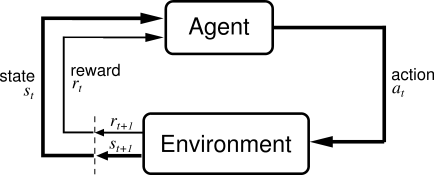
\includegraphics[width = 250pt]{agent_env.png}
  \caption{A visulization from the Sutton and Barto Book~\cite{Sutton1998}}
\end{figure}

\noindent The rewards signal replace the labels used in supervised learning. These rewards over time are
combined to form such targets in a variety of ways. A discount factor $\gamma \in [0,1]$ is introduced that
balances receiving immediate rewards against prioritizing long term rewards. Going closer towards 0 means
that immediate rewards gain high priority while the opposite is true when approaching 1.
The expected return at step $t$ is called $G_t$ and is an approximation of expected rewards when
starting in state $s_t$ and following policy $\pi$.
There are different ways of calculating an expected return, most notably Temporal Difference (TD) and Monte Carlo estimation~\cite{Sutton1998}.
Monte Carlo (MC) estimation defines $G_t$ as the discounted sum of all rewards received after time $t$.
\begin{equation}
    G_t^{MC} = \sum_{i=t}^T \gamma^{t-i+1} R_{i}
\end{equation}
This is an unbiased sample, but calculating our expected return this way leads to a variance of estimates.
TD($n$) methods are taking the next $n$ received rewards after step $t$ and then bootstrap a value. To bootstrap
a the value of a state we introduce a state value function $v_\pi : S \xrightarrow{} \mathbb{R}$. $v_\pi(s_t)$ is an estimate
of the discounted sum of rewards when starting in $s_t$.

\begin{equation}
    G_t^{TD(n)} = \gamma v_\pi(s_{t+n}) \sum_{i=t}^{t+n} \gamma^{t-i+1} R_{i+1}  
\end{equation}

\noindent Choosing a low value for $n$ will decrease variance, but increase bias. This is knows as the bias-variance tradeoff.
If the state value function is represented on the neural network, it is trained on the mean squared error between
its prediction of the state value $v_\pi(s)$ and the expected return $G_t$. If we are using a TD($n$) method the target
value is dependant on $v_\pi$, but does not use back propagate the loss through $G_t$. This is why these methods are sometimes
called semi-gradient methods~\cite{Sutton1998}. There is also other workarounds such as using a secondary model to predict
the target value and periodically copying over the weights~\cite{hessel2017rainbow}.\\

\noindent The algorithm which is chosen as the agent can be
separated into two major categories: On-Policy and Off-Policy. On-Policy algorithms need
to be trained on trajectories which are collected by following its policy $\pi$. Most On-Policy
models use a variaton of a policy gradient method~\cite{NIPS1999_464d828b} as update rule. The policys parameters are updated
with respect to their expected return. Sometimes a factor to weight different trajectories by their respective policys probabilities
is used, the importance sampling ratio $r$. For two policies $\pi$ and $b$ the importance sampling ratio is defined as:
\begin{equation}
    r : S\times A \xrightarrow{} \mathbb{R}
\end{equation}
\begin{equation*}
    r(s, a) = \frac{\pi(a|s)}{b(a|s)}
\end{equation*}
If appropriate for the selected agent this allows us to train on data obtained by other policies. The data for
On-Policy models can also only be used once for training, because after taking a gradient step the distribution $\pi(\cdot|s)$ changes
and therefore the data is no longer generated by our new $\pi$.\\
Off-Policy algorithms on the other hand can naturally be optimized
by data collected from any policy. Often this is true because Off-Policy methods use state-action value
functions $q_\pi : S\times A \xrightarrow{} \mathbb{R}$, instead of just state value functions. 
This means that while the value of function $v_\pi(s)$ is an average over all actions at the state $s$, $q_\pi$ does
not because the action is already selected. In discrete action spaces one can think about this as $v_\pi(s_t) = \sum_a \pi(a|s_t)
q_\pi(s_t, a)$, where in continuous action spaces the sum would be replaced by an integral over $a$.
The policy is then to simply select the action with the highest state action value.\\
Each of the two types of policies have their advantages. Off-Policy is a lot better in terms of
sample efficiency since data can not only be reused, but also data collected from other policies can be used.
On-Policy on the other hand usually learns a stochastic policy $\pi(\cdot|s) > 0$ which means that it keeps selecting 
different actions.\\
The act of selecting sub-optimal actions in order to find a more rewarding path to the goal is called exploration.
Taking the way that yielded the most reward in the past is called exploitation. These two create another
important tradeoff in RL, the exploration exploitation tradeoff. A policy will need to explore
sufficiently well before it keeps exploiting or it may never find the optimal trajectory. Optimal here means
the most reward collected.

\subsection{Arcade Learning Environment and Ms. Pac-Man}

The Arcade Learning Environment~\cite{DBLP:journals/corr/abs-1207-4708} has proven itself
as a good benchmark for RL agents. It withstood the test of time and is the de facto standard
for evaluating performance~\cite{DBLP:journals/corr/abs-1709-06009}. Best practices 
for using them include gray scaling the frames and stack 4 of them because some blinking
elements can only be seen if the environment is observed for this time. It is also
very common to rescale the frames to $84\times 84$, resulting in a state space consisting of $S = \{0,...,255\}^{4\times 84\times 84}$.
The full action space consists of 18 different action $A =\{0,...,18\}$, where only a single action
can be selected for each timestep $t$.\\
Of the over 50 games contained in the ALE we will take a closer look at the environment Ms. Pac-Man.
The player controls his character through a grid with walls and loses a life if a ghost
touches him. A player has three life in totals before we consider an episode to have ended.
In Ms. Pac-Man the player can obtain by rewards by collection dots and fruits on the map. Alternatively
an energy pill can be collected and ghosts can be killed for large rewards.\\
This leads to a challenging environment which can be tackled with a variety of different
plans i.e. prioritizing the collection of an energy pill and killing as many ghosts as possible
while largely neglecting the collection of rewards for picking up dots.

\begin{figure}
    \centering
    \subfloat[Beginning of an episode]{{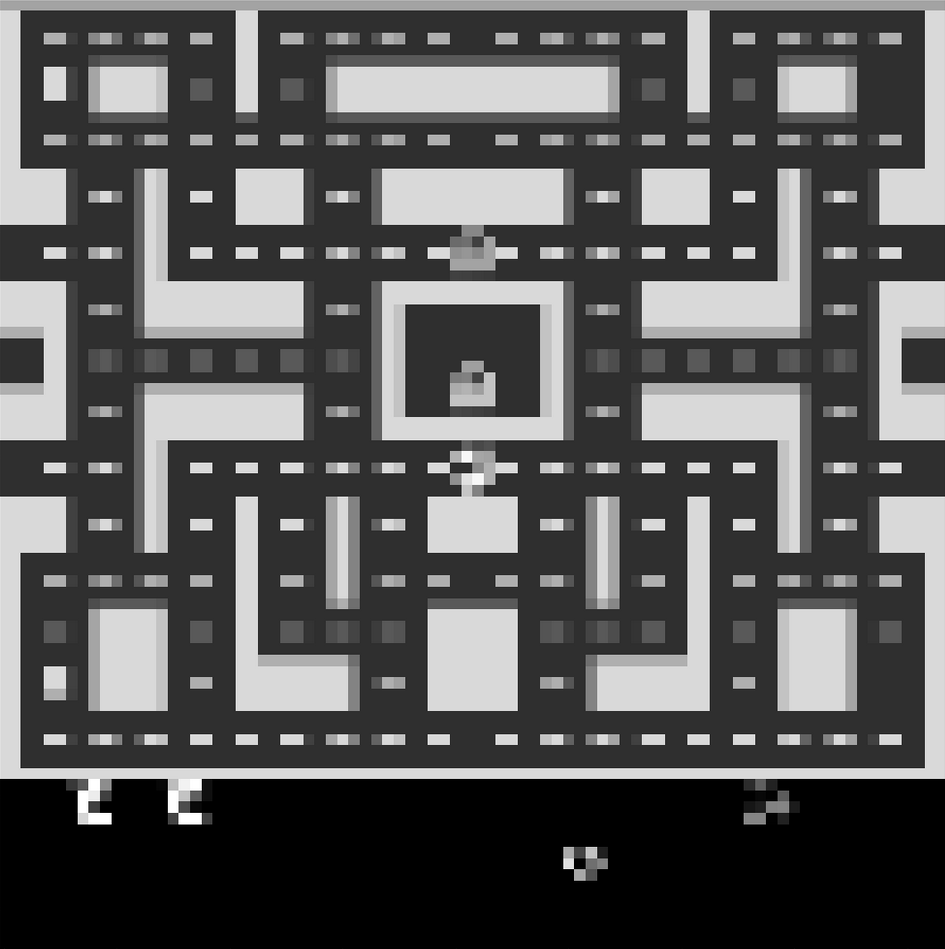
\includegraphics[width=5cm]{pacman_start.png} }}
    \qquad
    \subfloat[After 500 frames have passed]{{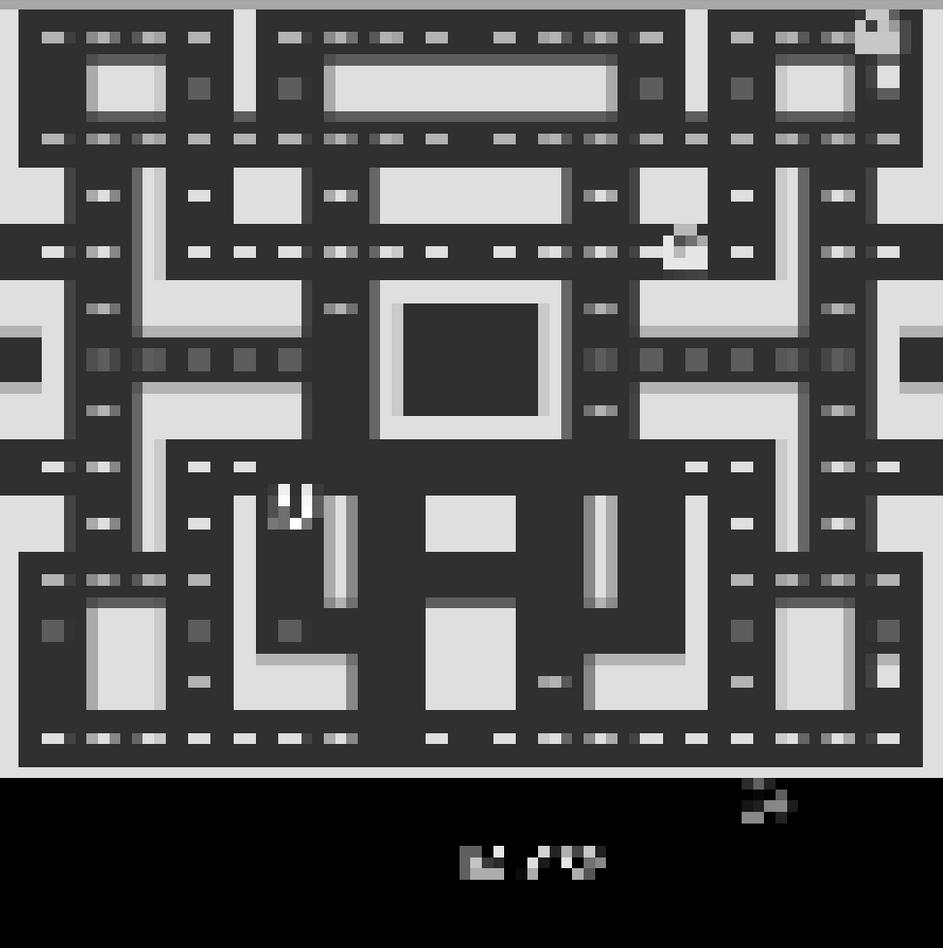
\includegraphics[width=5cm]{pacman.png} }}
    \caption{Two different frames of the game Ms. Pac-Man}
\end{figure}

\section{Trust Region Optimization Methods}

Trust Region Policy Optimization~\cite{pmlr-v37-schulman15} was first introduced by Schulman et al.
and aims to improve stability of training by limiting the Kullback–Leibler divergence $D_{KL}(\theta|\theta_{\text{old}})$
between the new policy $\pi_\theta$ and the old policy $\pi_{\theta_{\text{old}}}$. The KL divergence is a measure of how different
one distribution $\pi_{\theta_{\text{old}}}(a|s)$ is from another distribution $\pi_\theta(a|s)$.\\

\noindent This is achieved in~\cite{pmlr-v37-schulman15} by computing the second order derivative and adding 
a hard constraint to the weight update. 
\begin{equation}
    \theta_{\text{next}} \xleftarrow{} \arg \max_{\theta} {\mathcal L}(\theta_{\text{old}}, \theta) 
\end{equation}
\begin{equation*}
    \text{s.t.} \; {D}_{KL}(\theta|\theta_{\text{old}}) \leq \delta
\end{equation*}

\noindent where $\delta$ is the maximum KL divergence and ${\mathcal L}$ is called surrogate 
advantage. ${\mathcal L}$ is the estimated advantage weighted by the importance
sampling ratio between the new and the old policy. I define the importance sampling ratio $r(s, a)$ as:
\begin{equation}
    r : S \times A \xrightarrow{} \mathbb{R} 
\end{equation}
\begin{equation*}
    r(s, a) = \frac{\pi_{\theta}(a|s)}{\pi_{\theta_{\text{old}}}(a|s)}
\end{equation*}
where $s \sim S$ is one state drawn from the set of all states and $a \sim A$ is a
valid action selected from the set of all actions.

\noindent and our estimate for the advantage function $\hat A(s_t, a_t)$ at time step $t$ is
calculated via generalized advantage estimation~\cite{Schulmanetal_ICLR2016}. Here $\lambda$ is
the factor which controls the bias-variance tradeoff. A value near zero has typically a lot
less variance, but high bias. For a value near one it is the other way around.
Building a return this way is more flexible than using a n-step return method~\cite{DBLP:journals/corr/abs-2006-05990}.

\begin{equation}
    \hat A_\pi : S \times A \xrightarrow{} \mathbb{R} 
\end{equation}
\begin{equation*}
    \hat A_\pi(s_t, a_t)  = R_{t+1} + \gamma v_\pi(s_{t+1}) - v_\pi(s) + (1-d_t) \lambda \gamma \hat A_\pi(s_{t+1}, a_{t+1})
\end{equation*}

where $d_t \in \{0,1\}$ is an indicator whether time step $t$ was the last of an episode.
$v_\pi$ is the value function or critic of the algorithm.
The advantage function depends on the policy it is calculated for, so a subscript
indicates for which policy it is generated.

\begin{equation}
    {\mathcal L}_{\text{TRPO}}: S \times A \xrightarrow{} \mathbb{R}
\end{equation}
\begin{equation*}
    {\mathcal L}_{\text{TRPO}}(s, a) ={r(s, a) \hat A_{\pi_{\theta_{\text{old}}}}(s,a)}
\end{equation*}

\noindent This method stabilizes training but at the cost of computing the second order derivative
which requires a lot of compute.\\
To combat the additional required compute more modern trust region optimization methods
replace the hard constraint with a penalty term or clip the step size in some other way.

\subsection{Proximal Policy Optimization}
\noindent Proximal Policy Optimization~\cite{DBLP:journals/corr/SchulmanWDRK17} or PPO was first
introduced by OpenAI in 2017 and
has been a very popular On-Policy algorithm which supports both continuous and
discrete action spaces. OpenAI also emphasised that it has become their default
reinforcement learning algorithm due to its ease of use and good performance.\\
There are a few different Loss Terms shown in the paper, but I will focus on the main
suggestions, the PPO-Clip as it outperforms all other methods that use KL divergence penalty terms~\cite{DBLP:journals/corr/abs-2006-05990}.
The main idea behind PPO is to limit the step size as to avoid performance
collapse. To do so, one chooses an $\epsilon \in [0,1]$ as the policy clip ratio,
which is the maximal divergence from the old policy. This clipping is achieved
by construction the loss in such a way that the gradient for a divergence greater than $\epsilon$ is zero.
PPO updates its policy parameters $\theta$ via gradient ascent on the objective function ${\mathcal L}_{\mathrm{CLIP}}$:

\begin{equation}
    {\mathcal L}_{\mathrm{CLIP}}: S\times A \xrightarrow{} \mathbb{R}
\end{equation}
\begin{equation*}
    {\mathcal L}_{\mathrm{CLIP}}(s, a) = \mathrm{min}(r(s,a) \hat{A}_{\pi_\theta}, \mathrm{clip}(r(s,a), 1 - \epsilon, 1 + \epsilon)\hat{A}_{\pi_\theta})
\end{equation*}

\begin{figure}
    \centering
    \subfloat[$\hat A > 0$]{{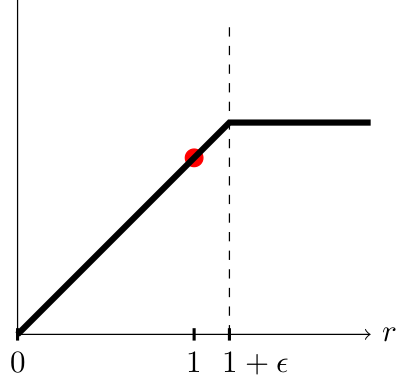
\includegraphics[width=5cm]{a_big_0.png} }}
    \qquad
    \subfloat[$\hat A \leq 0$]{{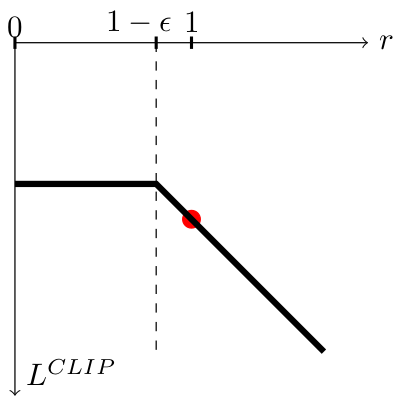
\includegraphics[width=5cm]{a_smal_0.png} }}
    \caption{Figure from original PPO paper visualizing the clipped objective~\cite{DBLP:journals/corr/SchulmanWDRK17}}
\end{figure}

\noindent Figure 3. show the effect of the clipped objective. Once the ratio
$r$ get bigger than the threshold $\epsilon$ the objective function get clipped and the gradient
beyond that point becomes zero. It is uncapped if the advantage is negative
and $r$ is positive because this means the negative advantage was scaled big because 
the selected, bad action became a lot more probable.\\
Because of this we obtain most of the benefits from TRPO but do not have
to compute the second order derivative.

\noindent The policy $\pi : S \xrightarrow{} A$ is represented by a neural network, which uses
the architecture of the original DQN-Paper~\cite{DBLP:journals/corr/MnihKSGAWR13}, consisting 
a convolution layer, which uses 16 filters of size 8 x 8 and stride 4,
followed by another, with 32 filter of size 4 x 4 with stride 2. The feature maps are then
flattened and transformed through a fully connected layer with 256 weight units.
The output layer is a fully connected layer as well and has one unit for every
action of the action space $A$ and is followed by the softmax function. 
An action is selected by sampling from this distribution and passed to environment.\\
To simplify notation we drop the $\theta$ when indexing policies, so $\pi$ refers to $\pi_\theta$ and
$\pi_{old}$ refers to the old policy $\pi_{\theta_{old}}$.
Trajectories generated by this network are used once for updating the policys
parameters before they are thrown out. At the time the trajectory is generated,
the probability of the selected action is saved and serves as the value for
$\pi_{old}(a|s)$ in the importance sampling ratio $r(s,a)$.\\
The value function $v_{\pi_\theta}(s_t)$ is also represented by a neural network and
is trained on the expected return $G_t = v_{\pi_{old}}(s_t) + \hat A_\pi(s_t,a_t)$
via mean squared error to the predicted value $\hat y = v_\pi(s_t)$. 
While the value function predicts the values if following the policy $\pi$ which is
indicated by the subscript, it has its own set of parameters $\psi$, which are updated
via gradient descent on its loss function $\mathcal{L}_{value}$.

\begin{equation}
    \mathcal{L}_{value}(\hat y, G_t) = MSE(\hat y, G_t)
\end{equation}

\noindent A PPO training phase, or policy phase consists of performing gradient steps according to Eq. 13
on all collected trajectory data and a critic training phase with gradient updated according to Eq. 14.
The critic and the policy network can share some layers, in
which case the value part is an additional neuron in the output layer
which acts as state value estimate. A benefit of this is from both,
the value loss function and the surrogate objective representations, which are mutual
beneficial for the tasks of each other are learned. The disadvantage of this is interference between
the two tasks.

\subsection{Phasic Policy Gradient}

Phasic Policy Gradient (PPG)~\cite{DBLP:journals/corr/abs-2009-04416} aims to the improve the
sample efficiency of PPO and get the best of both world from the shared-or-separate network
dynamic. This is achieved by using a shared-network architecture for the policy and an independent
critic network. This means that our policy has one more output neuron than there are valid actions.\\
In a new training phase, which is called the auxiliary phase, this extra value head is trained via
a combination of the value loss $\mathcal{L}_{value}$ and a behavior cloning loss. This loss limits divergence from the
old policy, while improving value estimation. The hyperparameter $\beta_{clone}$ controls
the size of the behavior cloning loss term and is usually set to 1.

\begin{equation}
    \mathcal{L}_{aux}(\hat y, G_t) = \mathcal{L}_{value}(\hat y, G_t) + \beta_{clone}\hat{\mathbb{E}}[KL(\pi, \pi_{old})]
\end{equation}
where $\hat y = \pi_{aux}(s_t)$ and $G_t = \pi_{aux}(s_t) + \hat A_\pi(s_t,a_t)$. The advantage function $\hat A$ in
$G_t$ is also dependent on the output value of the auxiliary head $\pi_{aux}$ and not on the critic $v_\pi(s)$.

\noindent In auxiliary phases the critic is also trained and updates its parameters $\psi$, but has no influence on the policy networks weights.
These phases work best if not performed too frequently as to not disturb
the policy learning. Often the value loss get scaled down or the maximum divergence from
the old policy is clipped via an approximation of the KL divergence. Due to auxiliary epochs being performed
infrequently this does not hurt runtime in a meaningful way.

\begin{figure}[htbp]
  \centering
  \includesvg[width = 250pt]{ppg.svg}
  \caption{PPG for 4 stacked Atari frames. The policy network $\pi_\theta$ with the extra value head in the output layer results in 19 total
  output neurons.}
\end{figure}

\newpage
\bibliography{refs}{}
\bibliographystyle{plain}
$$$$
\end{document}

\begin{comment}
Let $enc: \mathbb{R}^{n \times n} \xrightarrow{} \mathbb{R}^{m}$ be a neural network consisting of 
two convolution layers and a three layer MLP after the convolution. \newline
\end{comment}